\documentclass{beamer}
\usetheme{metropolis}           % Use metropolis theme
\setbeamercovered{transparent}

\usepackage{multicol}

\title{Writing a syllabus}
\date{\today}
\author{Mine \c{C}etinkaya-Rundel}
\institute{Sta 771S - Teaching Statistics}

\begin{document}
\maketitle
 
 
% -------------------------------------------------------------------

\section{A comprehensive syllabus}

% -------------------------------------------------------------------

\begin{frame}
\frametitle{What is a comprehensive syllabus}

A comprehensive syllabus:

\begin{itemize}
\item Sets the tone for the course.
\item Communicates what, when, and how students will learn.
\item Makes clear to students what they need to do in order to be successful.
\item Communicates expectations in terms of student responsibilities.
\item Deters misunderstandings about course policies.
\end{itemize}

\vfill

\tiny{Source: \url{http://www.cte.cornell.edu/teaching-ideas/designing-your-course/writing-a-syllabus.html}}

\end{frame}

% -------------------------------------------------------------------

\section{Components of a syllabus}

% -------------------------------------------------------------------

\begin{frame}
\frametitle{Components of a syllabus}

\begin{multicols}{2}
\begin{enumerate}
\item Title page
\item Course description
\item Course learning objectives
\item Course organization/logistics/format
\item Course requirements
\item Evaluation and grading policy
\item Course policies and expectations
\item Course calendar
\item Tips for success
\end{enumerate}
\end{multicols}

\end{frame}

% -------------------------------------------------------------------

\begin{frame}
\frametitle{Title page}

\begin{itemize}

\item Course number and title

\item Semester and year

\item Number of units

\item Meeting times and location

\item Instructor and TA information (e.g., name, office, office hours, contact information)

\item Pre-requisites and/or co-requisites

\item Required materials (e.g. textbook(s), technology)

\item Exam dates

\item Holidays

\end{itemize}

\end{frame}

% -------------------------------------------------------------------

\begin{frame}
\frametitle{Course description}

\begin{itemize}

\item A brief introduction to the course: scope and purpose

\item You can probably just use the official course description

\end{itemize}

\end{frame}

% -------------------------------------------------------------------

\begin{frame}
\frametitle{Course learning objectives}

\begin{itemize}

\item Itemized list of overall learning objectives for the course

\item Should be written using Bloom's taxonomy

\end{itemize}

\begin{center}
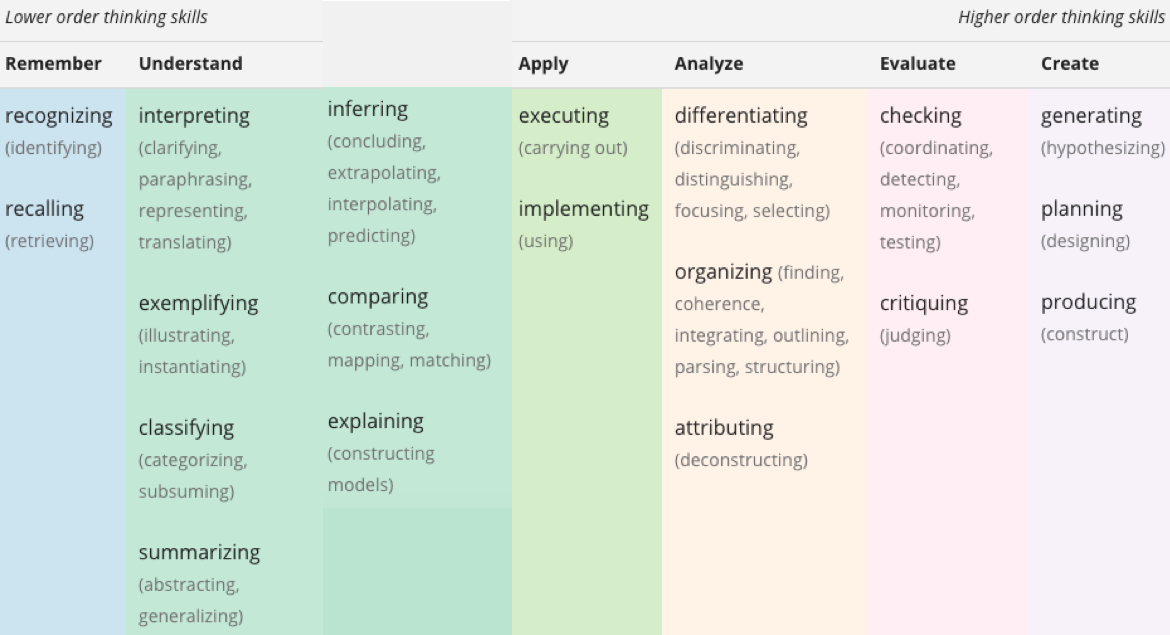
\includegraphics[width=0.9\textwidth]{blooms-taxonomy-revised.png}
\end{center}


\tiny{Source: \url{http://www.celt.iastate.edu/teaching/effective-teaching-practices/revised-blooms-taxonomy}}

\end{frame}

% -------------------------------------------------------------------

\begin{frame}[shrink]
\frametitle{Sample course learning objectives: STA 101}

\textit{
{\footnotesize
\begin{itemize}
\item Recognize the importance of data collection, identify limitations in data collection methods, and determine how they affect the scope of inference.
\item Use statistical software to summarize data numerically and visually, and to perform data analysis.
\item Have a conceptual understanding of the unified nature of statistical inference.
\item Apply estimation and testing methods to analyze single variables or the relationship between two variables in order to understand natural phenomena and make data-based decisions.
\item Model numerical response variables using a single or multiple explanatory variables.
\item Interpret results correctly, effectively, and in context without relying on statistical jargon.
\item Critique data-based claims and evaluate data-based decisions.
\item Complete a research project demonstrating mastery of statistical data analysis from exploratory analysis to inference to modeling.
\end{itemize}
}}

\end{frame}

% -------------------------------------------------------------------

\begin{frame}
\frametitle{Course organization/logistics/format}

\begin{itemize}

\item Describe the pedagogy

\item Outline what a week / unit looks like for students

\end{itemize}

\end{frame}

% -------------------------------------------------------------------

\begin{frame}[shrink]
\frametitle{Sample course format: Sta 101}

\textit{
{\footnotesize 
\begin{itemize}
\item The course is divided into seven learning units. 
\item For each unit a set of learning objectives and required and suggested readings, videos, etc. will be posted on the course website. 
\item You are expected to watch the videos and/or complete the readings and familiarize yourselves with the learning objectives. \item We will begin the unit with a readiness assessment: 10 multiple choice questions that you answer using your clickers in class. You will then re-take this assessment in teams. 
\item The rest of the class time will be split between discussion of the material and application exercises that you�ll complete in teams. 
\item Slides and other relevant materials for each class and lab will be available on the schedule page before each class. 
\item Videos and other relevant prep materials for each unit are also available on that page. 
\item Within each unit you will complement your learning with problem sets and labs, and wrap up each unit with a performance assessment.
\end{itemize}
}}

\end{frame}

% -------------------------------------------------------------------

\begin{frame}
\frametitle{Course requirements}

\begin{itemize}
\item What students will have to do in the course: assignments, exams, projects, performances, attendance, participation, etc. 

\item Describe the nature and format of each assignment and assessment and the expected length of written work.

\item Provide due dates for assignments and dates for exams.
\end{itemize}

\end{frame}

% -------------------------------------------------------------------

\begin{frame}
\frametitle{Course requirements}

\begin{itemize}

\item You must outline percentage distribution of graded work.

\item You might also want to say something about how final grades will be determined, e.g. curved or on a strict scale.
\begin{itemize}
\item Sample: \textit{Grades may be curved at the end of the semester. Cumulative numerical averages of 90 - 100 are guaranteed at least an A-, 80 - 89 at least a B-, and 70 - 79 at least a C-, however the exact ranges for letter grades will be determined after the final exam. The more evidence there is that the class has mastered the material, the more generous the curve will be.}
\end{itemize}

\item You should include instructions for accommodations for students with disabilities. There is likely official university language you can use for this.

\end{itemize}

\end{frame}

% -------------------------------------------------------------------

\begin{frame}
\frametitle{Course policies and expectations}

\begin{itemize}

\item A note on academic dishonesty must be included in your syllabus, you should use standard language that applies to your institution.
\begin{itemize}
\item Outline what the penalty might be for an academic dishonesty infraction.
\item Sample: \textit{Such incidences will result in a 0 grade for all parties involved as well as being reported to the Office of Student Conduct. Additionally, there may be penalties to your final class grade.}
\end{itemize}

\item Policy on absences, make up assignments and assessments must also be outlined.
\begin{itemize}
\item Tip: Stay clear of offering make up midterm exams, instead for excused absences plug in the final exam grade for the midterm. If a student cannot take the final exam on the scheduled date, they should drop the course.
\end{itemize}

\end{itemize}

\end{frame}

% -------------------------------------------------------------------

\begin{frame}
\frametitle{Course policies and expectations (cont.)}

\begin{itemize}

\item If you will be honoring regrade requests (this is recommended especially if multiple TAs are grading the work), outline a policy for regrades.
\begin{itemize}
\item Sample: \textit{Regrade requests must be made within one week of when the assignment is returned, and must be submitted in writing. These will be honored if points were tallied incorrectly, or if you feel your answer is correct but it was marked wrong. No regrade will be made to alter the number of points deducted for a mistake. There will be no grade changes after the final exam.}
\end{itemize}

\end{itemize}

\end{frame}

% -------------------------------------------------------------------

\begin{frame}
\frametitle{Course calendar}

\begin{itemize}

\item Provide a tentative schedule of topics to be covered.

\item List exact due dates for assignments (and do not move them up, though unforeseen circumstances might require that you delay them) and for exams (barring school closings do not ever move these). 

\item Note that your final exam date and time is likely determined by the university, not you. Find out where to get that information.

\end{itemize}

\end{frame}

% -------------------------------------------------------------------

\begin{frame}
\frametitle{Tips for success}

\begin{itemize}

\item Provide an itemized list of tips for success for your students.

\item These should be what you would tell a student if they came to your office asking ``How do you recommend I study for this course to do better?"

\end{itemize}

\end{frame}

% -------------------------------------------------------------------

\section{Introducing your syllabus in class}

% -------------------------------------------------------------------

\begin{frame}
\frametitle{Syllabus = contract}

\begin{itemize}

\item A syllabus is a like a contract for the course

\item When you hand it out to your students you agree to stick to it throughout the semester

\item And students, by staying in your course, agree to abide by the policies and expectations

\end{itemize}

\end{frame}

% -------------------------------------------------------------------

\begin{frame}
\frametitle{First day of class}

\begin{itemize}

\item It's a good idea to review the syllabus, however this can get tedious and boring for students

\item Try to keep this short

\item Consider a syllabus quiz

\end{itemize}

\end{frame}

% -------------------------------------------------------------------



\end{document}